% This is the Reed College LaTeX thesis template. Most of the work 
% for the document class was done by Sam Noble (SN), as well as this
% template. Later comments etc. by Ben Salzberg (BTS). Additional
% restructuring and APA support by Jess Youngberg (JY).
% Your comments and suggestions are more than welcome; please email
% them to cus@reed.edu
%
% See http://web.reed.edu/cis/help/latex.html for help. There are a 
% great bunch of help pages there, with notes on
% getting started, bibtex, etc. Go there and read it if you're not
% already familiar with LaTeX.
%
% Any line that starts with a percent symbol is a comment. 
% They won't show up in the document, and are useful for notes 
% to yourself and explaining commands. 
% Commenting also removes a line from the document; 
% very handy for troubleshooting problems. -BTS

% As far as I know, this follows the requirements laid out in 
% the 2002-2003 Senior Handbook. Ask a librarian to check the 
% document before binding. -SN

%%
%% Preamble

% The next lines tell TexShop to typeset with xelatex, and to open and save the source with Unicode encoding.
%!TEX TS-program = xelatex
%!TEX encoding = UTF-8 Unicode


\documentclass[12pt,twoside]{reedthesis}
% Packages are extensions to the basic LaTeX functions. Whatever you
% want to typeset, there is probably a package out there for it.
% Chemistry (chemtex), screenplays, you name it.
% Check out CTAN to see: http://www.ctan.org/
%%
%\usepackage{xeCJK}
%\setCJKmainfont{BiauKai}
\usepackage{graphicx,latexsym} 
\usepackage{amssymb,amsthm,amsmath}
\usepackage{longtable,booktabs,setspace} 
\usepackage{url} 
\usepackage{natbib}
\usepackage[protrusion=true,expansion=true]{microtype}
\usepackage{fontspec,xltxtra,xunicode,hyperref}
\defaultfontfeatures{Mapping=tex-text}
\setromanfont[Mapping=tex-text]{Minion Pro}
\hypersetup{
    backref=true,
    bookmarks=true,         % show bookmarks bar?
    unicode=false,          % non-Latin characters in Acrobat�s bookmarks
    pdftoolbar=true,        % show Acrobat�s toolbar?
    pdfmenubar=true,        % show Acrobat�s menu?
    pdffitwindow=false,     % window fit to page when opened
    pdfstartview={FitH},    % fits the width of the page to the window
    pdftitle={My title},    % title
    pdfauthor={Author},     % author
    pdfsubject={Subject},   % subject of the document
    pdfcreator={Creator},   % creator of the document
    pdfproducer={Producer}, % producer of the document
    pdfkeywords={keyword1} {key2} {key3}, % list of keywords
    pdfnewwindow=true,      % links in new window
    colorlinks=false,       % false: boxed links; true: colored links
    linkcolor=red,          % color of internal links (change box color with linkbordercolor)
    citecolor=green,        % color of links to bibliography
    filecolor=magenta,      % color of file links
    urlcolor=cyan           % color of external links
}
\urlstyle{same}
%\usepackage[hypcap]{caption}
 %\usepackage{} % other fonts are available like times, bookman, charter, palatino



\title{An Open Science Electrophysiology Study of\\Anxiety and Error Monitoring}
\author{Melissa D. Lewis}
% The month and year that you submit your FINAL draft TO THE LIBRARY (May or December)
\date{May 2013}
\division{Philosophy, Religion, Psychology, and Linguistics}
\advisor{Michael Pitts}
%If you have two advisors for some reason, you can use the following
%\altadvisor{Your Other Advisor}
%%% Remember to use the correct department!
\department{Psychology}
% if you're writing a thesis in an interdisciplinary major,
% uncomment the line below and change the text as appropriate.
% check the Senior Handbook if unsure.
%\thedivisionof{The Established Interdisciplinary Committee for}
% if you want the approval page to say "Approved for the Committee",
% uncomment the next line
%\approvedforthe{Committee}

\setlength{\parskip}{0pt}
%%
%% End Preamble
%%
%% The fun begins:

\begin{document}

  \maketitle
  \frontmatter % this stuff will be roman-numbered
  \pagestyle{empty} % this removes page numbers from the frontmatter

% Acknowledgements (Acceptable American spelling) are optional
% So are Acknowledgments (proper English spelling)
    \chapter*{Acknowledgements}

Arianna, Natasha, Annelyse, Rose, and Juliet, the women with whom I've shared a home, victories, setbacks, and a lot of Thai food: from you I learned how to love fearlessly and how to persist.

Michael, my advisor: I first learned to be practically and optimistically critical of science from you, and I am grateful for how you have enriched my academic and intellectual experience at this school. 

Reed College: you are an improbable assembly of administrators, faculty, staff, and students. I am humbled and galvanized by my time with you, and I will always work to give to others as you have given to me.

Everything I can say I've accomplished is a product of many people's magnanimity, long emails, Trader Joe's gift cards, copyediting, mackerel, wisdom, flowers, crushing hugs, jokes, stories, surprise visits, and cat pictures. You inspire me to be present, stubborn, and gracious. I hope my life reflects your benefaction.

% The preface is optional
% To remove it, comment it out or delete it.
    \tableofcontents
% if you want a list of tables, optional
    \listoftables
% if you want a list of figures, also optional
    \listoffigures

% The abstract is not required if you're writing a creative thesis (but aren't they all?)
% If your abstract is longer than a page, there may be a formatting issue.
    \chapter*{Abstract}

Replicability is essential to scientific progress, but published research findings are less likely to be replicated every year. This experiment was both a replication of a previous research finding and an extension of its associated questions. The original experiment investigated whether an event-related potential called the error-related negativity (ERN) indexed motivational or emotional aspects of error monitoring. They did so by investigating whether it correlated to a physiological index of defensive motivation, the startle response to a loud auditory stimulus as measured by electromyography (EMG) at the orbicularis oculi muscle. This experiment replicated increased startle magnitude following errors compared to correct responses, suggesting a relationship between defensive motivation and error detection. This experiment also replicated the finding of an ERN with the same scalp distribution of the original study and in the same time frame (peaking roughly 50ms after response). However, it did not find a correlation between the magnitude of the startle response and the amplitude of the ERN, as the original study found. As an extension, this experiment manipulated state anxiety with a feedback system based on points. It also used the Spielberger State-Trait Anxiety Inventory to examine whether there was a relationship between self-reported state and/or trait anxiety and the ERN and/or startle response. The results showed that trial type modulated startle response. However, state anxiety could not be teased out for its effect on startle or the ERN, and there was no correlation between ERN and startle. No relationship between trait anxiety and the ERN or the startle response was found.

	
	\chapter*{Dedication}

To Charleston Elementary, convergence of blossoming trees, tetherball, and teachers who said that making the world a better place is a perfectly viable career option.

  \mainmatter % here the regular arabic numbering starts
  \pagestyle{fancyplain} % turns page numbering back on

%The \introduction command is provided as a convenience.
%if you want special chapter formatting, you'll probably want to avoid using it altogether

\chapter*{Introduction}
         \addcontentsline{toc}{chapter}{Introduction}
	\chaptermark{Introduction}
	\markboth{Introduction}{Introduction}
	% The three lines above are to make sure that the headers are right, that the intro gets included in the table of contents, and that it doesn't get numbered 1 so that chapter one is 1.

% Double spacing: if you want to double space, or one and a half 
% space, uncomment one of the following lines. You can go back to 
% single spacing with the \singlespacing command.
% \singlespacing
%\doublespacing
\onehalfspace

	\section[The Neural Basis of Error Monitoring and Defensive Motivation]{The Neural Basis of Error Monitoring and \protect\\ Defensive Motivation}
	
		\subsection{Error Monitoring}
		The mechanisms by which people monitor and correct for errors remain rich areas of investigation in neuroscience and psychology in general.  Related to executive control, detection of errors during response monitoring -- whatever its underlying mechanisms -- consistently proves aversive \citep{leue_modulation_2012}. One prominent model of error monitoring, the integrative account, posits that the aversiveness arises from anticipation of greater cognitive demand \citep{botvinick_conflict_2007}. Another model, revised reinforcement sensitivity theory (rRST), describes the aversive nature of errors as originating in anticipation of negative consequences \citep{corr_reinforcement_2004}. Evidence from experiments manipulating task complexity points to a significant role of expectation of cognitive load \citep {leue_modulation_2012}. However, experiments manipulating incentives and performance import lend credence to rRST  \citep{weinberg_integrating_2011,bush_cognitive_2000}. These two models seem not be mutually exclusive and error aversion may be supported by simultaneously viable mechanisms \citep{bush_cognitive_2000}. One of the key features shared by both of these theories is the central role of defensive motivation in error monitoring and detection.
		\subsection{Defensive Motivation} 
		In the context of error monitoring, defensive motivation is thought to arise as a response to a commission error as a means of improving diligence and mitigating future errors. Evidence for this comes from a variety of experimental manipulations, including reward incentives and punishments \citep{leue_modulation_2012,weinberg_integrating_2011}. Additionally, insofar as defensive motivation is yoked to affective states like anxiety, evidence for a relationship between affective states and error comes from experiments measuring and manipulating state anxiety and also measuring the more stable trait anxiety \citep{hajcak_what_2012}. Measures of defensive motivation include skin conductance and startle response \citep{hajcak_errors_2008}.
		\subsection{The ERN and Startle}
		The error-related negativity (ERN) is a particular type of event-related potential (ERP). ERPs reflect brain activity corresponding to specific sensory, cognitive, or motor events and are small signals embedded in larger ongoing electrical activity measured at the scalp via electroencephalography (EEG).  During a recording of EEG, electrodes at the scalp are thought to be recording the voltage resulting from the summation of dipoles. Dipoles are are spatially proximal pairs of positive and negative electrical charges originating in postsynaptic potentials \citep{luck_introduction_2005}. Because of the convoluted nature of the cortex it is unclear what relationship these charges have to the function or location of the neural region underlying them. It is clear, though, that this voltage fluctuation occurs as a consequence of the activity of postsynaptic potentials, because when excitatory neurotransmitters are released at apical dendrites of pyramidal cells in the cortex, i.e. presynaptic terminals, it causes positive ions to flow into the postsynaptic neuron. This leaves the charge outside of the cell relatively negative. Then current flows out of the cell body and basal dendrites, creating a net positivity.
		
The ERN is a negative-going ERP component peaking roughly 50-100 milliseconds after a commission error (Figure~\ref{fig:hajcakERN}) and is usually found over the frontal-central scalp \citep{falkenstein_effects_1991}. While it is often difficult to determine the source of an ERP component, source localization algorithms whose purpose is identification of scalp-recorded ERP neural generators indicate that the source of the ERN is in the midline prefrontal cortex, where the anterior cingulate cortex (ACC) is located. Additionally, measurement of local field potentials in the ACC of monkeys find increased firing when the animals make an error, at a similar time frame as the ERN \citep{bush_cognitive_2000}.

Experiments have found a positive relationship between ERN amplitude and a variety of other phenomena, including diagnosis of obsessive-compulsive disorder, diagnosis of generalized anxiety disorder, and higher ratings of anxiety irrespective of diagnoses \citep{weinberg_integrating_2011}. Such findings prompted some researchers to suggest that increased ERN itself might be a predictive marker of anxiety and disorders thereof \citep{hajcak_what_2012}.
		\begin{figure}[h]
	% the options are h = here, t = top, b = bottom, p = page of figures.
	% you can add an exclamation mark to make it try harder, and multiple
	% options if you have an order of preference, e.g.
	   
	       \centering
	    % DO NOT ADD A FILENAME EXTENSION TO THE GRAPHIC FILE
	    \includegraphics{hajcak_ERN_voltage}
	     \caption[Mean event-related potentials time-locked to correct and erroneous responses in Hajcak 2012]{Mean event-related potentials time-locked to correct and erroneous responses at electrode FCz (left). This graph plots voltage over time, where the response occurs at 0 milliseconds (ms). The error-related negativity (ERN) is observed as a sharp negative deflection that peaks around 50 ms (illustrated by the gray bar) after the commission of a mistake.The voltage difference between errors and correct responses in the time window of the ERN can be plotted over the scalp (right); the ERN is maximal at the frontal-central midline of the scalp. Caption also from Figure 1 of Hajcak, 2012}
	 \label{fig:hajcakERN}
	\end{figure}

		\subsection{State versus Trait Anxiety} \label{sec:anxiety}

		
A consensus as to the definition of emotions in general is still absent in the literature, but in the context of the current study it makes sense to adopt a view seating emotion in motivational states and to define their parameters as 1) direction away from or toward a stimulus, and 2) magnitude of motivation, commonly referred to as valence and arousal respectively \citep{luck_oxford_2012}.

Most generally, state anxiety is differentiated from trait anxiety in its duration and relationship to stimuli: state anxiety can be a reaction to a threatening stimulus, but trait anxiety can be sustained in the absence of a particular cause \citep{endler_state_2001}. One measure used to differentiate between these is a 40-item questionnaire called the Spielberger State-Trait Anxiety Inventory (STAI). Though it is among the longest- and most widely-used studies differentiating between these types of anxiety, it remains unclear whether the questions identifying trait anxiety are also measuring depression \citep{bieling_state--trait_1998}. However, their comorbidity and shared mechanisms -- neurophysiological and even genetic -- make these generally difficult to isolate \citep{andrews_bright_2009}.

Anxiety is uniquely suitable for ERP studies because other states are likelier to decay over as many trials as are necessary to obtain a meaningful signal. ERPs can serve as a useful complement in discerning causal relationships between stimuli and response \citep{luck_oxford_2012}, because they can be used to measure physiological arousal that would accompany an anxious, but not a depressed, affect that cannot be dissociated in a questionnaire \citep{gros_psychometric_2007}.

Evidence exists for a significant role of state anxiety in increasing vigilance in cognitive tasks. Activity increases in the same region of the brain (the right ventrolateral prefrontal cortex) during both exposure to threatening stimuli and during difficult vigilance tasks, e.g. when search stimuli are relatively difficult to distinguish from background stimuli, or when search criteria must be held in working memory for a long period of time \citep{aron_inhibition_2004}. Similar to such evidence for potential adaptiveness of state anxiety, evidence exists for an adaptive role of the longer-term trait anxiety as well. The analytical rumination (AR) hypothesis posits an adaptive role for the frequently comorbid trait anxiety and depression in attentional control and sustained analysis of complex issues \citep{andrews_bright_2009}.
	\section{Open Science}
		\subsection{Historical Precedence}

Most published research findings, whether in medical or psychological science, are not replicable \citep{ioannidis_why_2005}. Many causes appear to contribute to nonreplication, including demands for novel positive findings \citep{taubes_epidemiology_1995,fanelli_negative_2011}. Additionally, false positives abound because of the margin allowed by the \textless.05 \textit{p}-value criterion for publication \citep{ioannidis_why_2005}. Most retractions are due to error, rather than outright fraud. See Table~\ref{tab:retraction}.

\begin{table}[h]
\caption[Reasons for Retraction of 742 Papers, 2000 - 10.]{Reasons for Retraction of 742 Papers, 2000 - 10. Source of Retractions: PubMed. Adapted from Steen 2010.} 
\begin{center} 
\begin{tabular}{l l l} 
\toprule % a horizontal line, slightly thicker than \hline, depends on the booktabs package
Reason for retraction & Retracted paper, n(\%) & IF, mean (SD) \\ % the first row of the table. Separate columns with ampersands and end the line with two backslashes. An environment begun in one cell will not carry over to adjacent rows.
  \midrule % another horizontal line
\bf{Fraud} & & \\ % another row
Fabrication & 111 (15.0) & 9.70 (11.49) \\
Falsification & 98 (13.2) & 8.01 (8.33)\\
\bf{Error} & & \\
Scientific mistake & 234 (31.5) & 10.60 (10.66) \\
Duplicate publication & 117 (15.8) & 3.18 (2.63) \\
Plagiarism & 107 (14.4) & 2.31 (1.90) \\
Ethical violations & 76 (10.2) & 5.74 (8.51) \\
Unstated reasons & 61 (8.2) & 5.08 (8.82) \\
Journal error & 27 (3.6) & 2.66 (2.21) \\
\bottomrule % yet another horizontal line
IF = impact factor
\end{tabular}
\end{center}
\label{tab:retraction} % labels are useful when you have more than one table or figure in your document. See our online documentation for more on this.
\end{table}

Additionally, the structure of professional science today emphasizes publications, and those publications hinge on novel positive findings. These publications are the arena of labs' competition for funding. Meta-analyses find that statistically significant results are three times more likely to be published than papers affirming null results \citep{jennings_publication_2011}. Because it is circular to explain this disparity being caused by experimenters' desires to submit significant findings, it is also important to consider the roles that reviewers and editors have in preferring those significant findings. Not only are concurrent articles differentially prioritized according to whether they report positive results, but positive results are privileged if they are novel. This privileging occurs irrespective of the frequency of null findings (i.e. failure to replicate), a phenomenon called latent bias. Finally, retractions of improperly reported positive findings are higher among more influential journals \citep{fang_retracted_2011} as indexed by their impact factor, i.e. how frequently their recent articles are being cited in other journals. 

Transparency would address methodological problems across kind and degree, from innocuous problems of standardizing experimental conditions and protocols to outright forgery. Thanks to the internet, researchers interested in implementing these practices are able to coordinate. Some endeavors are ostensibly more social, e.g.\ ResearchGate, of note because it is a place where researchers can post their research for free, at least for articles published in journals that allow this. Other potential solutions are concerned more with methodology, as in Figshare, a site where every component of the scientific process, including methods and datasets, can be shared publicly for free and assigned their own digital object identifiers (DOIs) to be used for citation.

Reaching consensus that science needs to be more open is the first and simplest obstacle to proliferating the practice. Adoption in the community and standardization within and among practices proves to be much more complex. While analyses of extant publications are important in both understanding the kind and extent of such problems, an important complement to these endeavors is systematic replication. The Center for Open Science was founded to integrate these solutions.
		
		\subsection{The Center for Open Science}
		
The Center for Open Science has three primary activities: the Open Science Collaboration (OSC), the Open Science Framework (OSF), and the Reproducibility Project (RP).  The Open Science Collaboration is the broader community interested in open practices, spanning scientific disciplines and open-source developers. The OSF is focused on developing infrastructure for collaboration, including version control, a centralized place for sharing and finding experimental materials, documenting work, and standardizing workflow. The RP is focused on both the rate of reproducibility and how this rate can be improved.
		
		\subsubsection{The Reproducibility Project}
		
At the time of this writing, over 100 scientists have joined a single endeavor to replicate experiments published in three prominent psychological science journals: \textit{Psychological Science}, the \textit{Journal of Personality and Social Psychology}, and the \textit{Journal of Experimental Psychology: Learning, Memory, and Cognition}. The purpose is not just to test reproducibility of published research findings, but to develop a methodology to improve it \citep{open_science_collaboration_open_2012}.

Most studies come from the fields of social and cognitive psychology because they do not require specialized equipment and are less expensive, and most replications require undergraduate subjects \citep{carpenter_psychologys_2012}. Though such a homogeneous research population presents its own problems, a significant advantage exists in limiting costs of such studies because it serves dual purposes, including training \citep{frank_teaching_2012}.

Participation in the Reproducibility Project entails collaboration with other members to develop strategies for adhering as closely to the original study as possible given inevitable differences between the respective labs and their access to materials. Because the course of the replication will be transparent, participating researchers will send a report outlining their plan for replication according to a template. See Appendix C:~\nameref{chap:RPreport} for a comparison between methods in this and the original study, as the methods in the following chapter describe only the methods for this replication.

\chapter{The Replication}
    	\section{Methods}
		\subsection{Participants}
Participants were 30 undergraduate students aged 18-35 (18 female, 12 male). Human Subjects Research Committee approval was obtained before the study began.
		\subsection{The Task}
Participants performed a flanker task in which they viewed five horizontally aligned arrows (< < > > >) on a computer screen. On each trial, participants were to specify the direction of the central arrow with the click of a left or right mouse button. Whether the central arrow was aligned with flankers was pseudorandomly chosen and of equal frequency. Trials on which central and flanker arrows were aligned will hereafter be called compatible, while trials on which the central and flanker arrows were not aligned will hereafter be called incompatible.

Each participant first performed one practice block of 30 trials followed by eight additional blocks of 30 trials. Stimuli (i.e. the arrows) were presented for 200 ms with an intertrial interval (ITI) that varied pseudorandomly from 500 to 1000 ms. At the end of each of these blocks, participants saw on the screen one of three messages according to performance: if 75\% accurate or below, they saw ``Please try to be more accurate"; if above 90\% they saw ``Please try to respond faster"; if between these levels of accuracy, they saw ``You're doing a great job." The purpose of this feedback was to encourage participants to balance speed and accuracy, and also to induce enough errors to examine for the ERN.
		\subsection{Errors and EEG}
While performing this task each participant was monitored for his or her electroencephalographic (EEG) and electromyographic (EMG) activity using the EasyCap electrode cap and BrainAmps Standard system (Brain Products, Gilding, Germany). Recordings were taken from 96 scalp electrodes at equidistant positions as well as from two reference electrodes placed on the left and right mastoids. Electrooculogram (EOG) from blinks and other eye movements were recorded from four facial electrodes placed approximately 1 cm: above the right eye, below the right eye, left of the left eye, and right of the right eye. All bioelectric signals were digitized on a laboratory microcomputer using Recorder software (Brain Products). Sampling was at 1000 Hz.

Offline analysis was performed using Brain Vision Analyzer software (Brain Products, Gilching, Germany). Data were referenced to the numeric mean of the mastoids and band-pass filtered with cutoffs of 0.1 and 30 Hz. EEG was segmented for each trial, beginning 200 ms before response and continuing for 800 ms. It was corrected for blinks and eye movements using EMCP \citep{gratton_new_1983}.  The ERN was defined as the average activity in a 0- to 100-ms window following response onset on error trials, but it generally peaks approximately 50 ms following commission of an error. The ERN was statistically evaluated using R, with Greenhouse-Geisser correction applied to p values associated with multiple degrees of freedom, repeated measures comparisons.
		\subsection{Startle and EMG}
Startle probes consisted of a 50-ms 99-dB white noise with instantaneous onset 300ms after response. They were presented on 10\% of all trials in the practice block. In the eight blocks following practice, they were presented on 4\% of correct trials preceded by correct trials (called ``correct unpredictable" because the presentation of the startle probe is relatively unlikely), 50\% of error trials, and 50\% of correct trials following errors (also called ``correct predictable" as the probability of 50\%, though random, is a much higher rate than that of the other correct trial type).

Startle response was measured with two electrodes placed approximately 12 mm apart under each participant's left eye on the orbicularis muscle. Startle response EMG data was band-pass filtered (28---512 Hz; 24 dB/octave roll-off), rectified, then low-pass filtered at 30 Hz (24 dB/octave) and baseline-corrected. Response magnitude and latencies were quantified according to a peak in the 20- to 120-ms window after the startle probe was presented. It was statistically evaluated using R, with Greenhouse-Geisser correction applied to p values associated with multiple degrees of freedom, repeated measures comparisons.
	\section{Results}
	\subsection{Startle}
On average, participants made 36.13 (\textit{SD} = 19.70) errors. As in the original study, the magnitude of the startle response differed as a function of trial type, \textit{F}(2,56)=9.36, \textit{p} < .001 (see Figure~\ref{fig:startlebar}). Follow-up \textit{t} tests found that startle magnitude was greater following errors than following either subtype of correct trial, whether predictable, \textit{t}(28) = 3.79, \textit{p} < .001, or unpredictable \textit{t}(28) = 2.90, \textit{p} < .01. Additionally, there was no significant difference between correct unpredictable and correct predictable trials, \textit{t}(28)=-1.7025, \textit{p} > .09. There was no correlation between number of errors and error-potentiated startle magnitude, \textit{r} = -.10, \textit{p} > .5.  As in the original study again the latency of startle response was shorter for predictable (for error: \textit{M} = 62ms, \textit{SD} = 5.8ms and for correct predictable: \textit{M} = 62.7ms, \textit{SD}=4.7ms) than for unpredictable trials (\textit{M} = 64.4, \textit{SD} = 6.6ms), but the difference was not significant \textit{F}(2,56) = 2.81, \textit{p} > .05. %<number of trials removed for each startle type on average to be calculated>
	\begin{figure}[h]
	% the options are h = here, t = top, b = bottom, p = page of figures.
	% you can add an exclamation mark to make it try harder, and multiple
	% options if you have an order of preference, e.g.
	   
	  \centering
	    % DO NOT ADD A FILENAME EXTENSION TO THE GRAPHIC FILE
	  \includegraphics{bargraph_comparison_v3}% figure 1.1
	   \caption[Comparison of mean startle magnitude by trial type from original and replication study]{Comparison of mean startle magnitude by trial type from original and replication study. Error bars represent the 95\% confident interval. Asterisks indicate significant differences between trial type, \textit{p} < .01. Caption adapted from Figure 1 of \citep{hajcak_errors_2008}}.
	   \label{fig:startlebar}
	   \end{figure}

	\subsection{The Error-related Negativity}
	The ERN is often measured as the difference between ERPs for correct and error trials (here measured in the 0-100ms window following response). The presence of the ERN is assessed by comparing this difference wave to 0. Because the presence of the ERN was investigated in the original article at a single electrode site, FCz, it was investigated here at the closest analogous site in the 96-channel setup, electrode 2. At electrode 2, a one-sample \textit{t} test found that ERN amplitude (0-100ms post-response) differed significantly from 0, \textit{t}(29) = -6.85, \textit{p} < .001. Figure~\ref{fig:comparisonERN} depicts the scalp topography of the ERN on the left and the grand average ERP waveform for correct and error trials on the right. The peak at 400ms in the replication study ERPs is absent in the original study. While the nature of this extra peak is as yet undetermined, its timing is such that it could be a post-auricular muscle (or PAM) response, which is well-documented electrical activity evoked in the muscle behind the ear (on the mastoid) following a brief auditory stimulus \citep{obeirne_basic_1999}. This signal would appear in most scalp channels, even one on the top of the head, because they are all referenced to the mastoid electrodes.  Further supporting this possibility is the difference in amplitude of this peak between correct and error trials. The probability of presentation of the auditory stimulus was a combination of 4\% for correct unpredictable and 50\% of correct predictable trials, which would result in fewer presentations than for just error trails because that probability was always 50\%. Because the original study also referenced to the mastoids after recording, it is unclear why the PAM response does not also appear in their data.
	
	\begin{figure}[t]
	\label{fig:comparisonERN}
	% the options are h = here, t = top, b = bottom, p = page of figures.
	% you can add an exclamation mark to make it try harder, and multiple
	% options if you have an order of preference, e.g.
	    \centering
	    % DO NOT ADD A FILENAME EXTENSION TO THE GRAPHIC FILE
		\includegraphics{fig2sanscor}%figure 1.2
		\caption[Comparison of mean event-related potentials time-locked to correct and erroneous responses between the original and replication studies]{Comparison of mean event-related potentials time-locked to correct and erroneous responses at analogous electrode sites FCz and 2 between the original and replication studies, respectively (left). The graph (right) plots voltage over time, where response occurs at 0 milliseconds (ms). The error-related negativity (ERN) is a sharp negative deflection that peaks around 50 ms after the commission of a mistake, and its amplitude is calculated as the voltage difference between errors and correct responses in a 100-ms time window. The ERN is plotted over the scalp (left) and is maximal at the frontal-central midline of the scalp.}
		
	\end{figure}

	\subsection{Error-potentiated Startle and the Predictive Value of the ERN}
	Analogous to finding the ERN by subtracting correct from error trials, the original authors defined the error-potentiated startle (EPS) as the startle magnitude after errors minus the average startle magnitude of correct predictable and correct unpredictable trials. The original study found that the ERN predicted the potentiation of startle response, but the current study failed to replicate this finding, \textit{r} = -.28, \textit{p} > .12. %See Figure~\ref{fig:correlation} for comparison.\\	
	\begin{figure}[h]
	% the options are h = here, t = top, b = bottom, p = page of figures.
	% you can add an exclamation mark to make it try harder, and multiple
	% options if you have an order of preference, e.g.
	
	   
	       \centering
	    % DO NOT ADD A FILENAME EXTENSION TO THE GRAPHIC FILE
	    \includegraphics{corplot2}%figure 1.3
	     \caption[Comparison of correlation of ERN amplitude and error-potentiated startle magnitude between original and replication studies]{Left: original scatterplot depicting the magnitude of the error-potentiated startle as a function of ERN amplitude. Right: replication findings, not significant (\textit{p} > .05)}
	 \label{fig:correlation}
	\end{figure}
	\section{Discussion}
Results for the ERN and for startle aligned closely with those of the original study, but the correlation between the EPS and ERN did not hold. See Figure~\ref{fig:correlation} for comparison of scatterplots between the original and replication studies. However, the original author has also faced difficulty replicating this finding \citep{riesel_press_2013}. A significant correlation between EPS and the ERN emerged only after the authors performed exploratory post-hoc analyses and formed two subgroups of participants based on a median split of participants into groups with high and low amplitude relative to -8.25$\mu$V. A correlation between ERN amplitude and startle magnitude was found among those participants whose ERN amplitude was relatively high, i.e. above the median, \textit{r} = -.60, \textit{p} < .05. Dividing participants in the current study along the median (5.85$\mu$V) also generated a significant correlation, \textit{r} = -.64, \textit{p} < .001. See Figure~\ref{fig:split}.

	\begin{figure}[h]
	       \centering
	    % DO NOT ADD A FILENAME EXTENSION TO THE GRAPHIC FILE
	    \includegraphics{split2}
	     \caption[Comparison of correlation of ERN amplitude and error-potentiated startle magnitude before and after median split]{Left: Replication scatterplot depicting the magnitude of the error-potentiated startle as a function of ERN amplitude, r = -.27, \textit{p} > .05. Right: correlation plot including only those participants whose ERN amplitudes were above median 5.85$\mu$V).}
	\label{fig:split}
	\end{figure}

While this median split led to significant correlations in both studies, the scatterplots from each study reveal a potential outlier. When the array of values for the ERN and for the EPS are investigated independently for the value with the largest difference from the sample mean, each is found to belong to the same participant (\textit{z}(ERN) = -2.98, \textit{z}(EPS) = 2.95). When this participant is removed, the correlation fails to be significant even when participants are split by the median, \textit{r} = .09, \textit{p} > .75. See Figure~\ref{fig:outlier} for a comparison of correlations before and after removal of this potential outlier.

	\begin{figure}[h]
	       \centering
	    % DO NOT ADD A FILENAME EXTENSION TO THE GRAPHIC FILE
	    \includegraphics{outlier2}
	     \caption[Comparison of correlation of ERN amplitude and error-potentiated startle magnitude after median split, with and without outlier]{Left: Scatterplot depicting the magnitude of the error-potentiated startle as a function of ERN amplitude in participants whose ERN was of relatively high amplitude, r = -.60, \textit{p} > .05, outlier circled. Right: Same as left, but without outlier.}
	 \label{fig:outlier}
	\end{figure}
	
\chapter{The Extension}
    	\section{Methods}
Following the replication, participants were asked to complete the state-trait anxiety inventory (STAI) (see~\nameref{sec:anxiety}). The task and stimuli were identical to that of the replication.

Additionally, participants performed the task in another 8 blocks of 30 trials for each of two conditions. In the low anxiety condition, subjects received +2 points for correct responses faster than their average RT, +1 points for correct responses slower than their average RT, and -1 points for incorrect responses. In the high anxiety condition, +1 point was received for correct/fast trials, -1 point for correct/slow trials, and -2 points for incorrect trials. The order in which each of these conditions was presented was counterbalanced between subjects. By manipulating points, we sought to manipulate state anxiety. Subjects were informed at the outset that the fastest, most accurate participant would win \$75. Participants filled out an identical STAI form following the extension trials as well.
	
	\section{Results}
		\subsection{Anxiety}
There was no significant difference between trait scores reported by participants before and after anxiety manipulation \textit{t}(24) = -.49, \textit{p} > .63. There was also no significant difference in state anxiety before and after the anxiety manipulation, \textit{t}(24) = 1.09, \textit{p} > .28. Trait and state anxiety were not significantly correlated before anxiety manipulation, \textit{r}=.28, \textit{p} > .14. Following anxiety manipulation, however, trait and state anxiety are significantly correlated, \textit{r}=.62, \textit{p} < .01.

		\subsection{Anxiety and Electrophysiological Measures}
		
There was no effect on ERN of anxiety manipulation (\textit{F}(1,25) = 1.10, \textit{p} > .30), order (\textit{F}(1,25) = 0.40, \textit{p} > .54) or interaction between the two  (\textit{F}(1,25) = 1.60, \textit{p} > .22). There was no effect on EPS  of anxiety manipulation (\textit{F}(1,25) = 1.71, \textit{p} > .20), order (\textit{F}(1,25) = 4.05, \textit{p} > .05) or interaction between the two  (\textit{F}(1,25) = 0.49, \textit{p} > .49).

Because the EPS magnitude is calculated by subtracting the average startle magnitude of correct trials from error trials, it may be obscuring differential effects of anxiety manipulation on startle magnitude within these trial types. An ANOVA examining effects on startle magnitude within trial type (error, correct predictable, or correct unpredictable) and anxiety condition (low or high) and between the order of anxiety conditions (low to high or high to low) found main effects of anxiety condition (\textit{F}(1,25) = 5.39, \textit{p} < .01) and trial type (\textit{F}(2, 50) = .4.96, \textit{p} < .01) (see Figure~\ref{fig:ext_startle}) , and an interaction between order and anxiety condition (\textit{F}(1, 25) = 12.29, \textit{p} < .01). This ANOVA found no effect of order (\textit{F}(1, 25) = 0.90, \textit{p} > .35). Additionally, interactions between order and trial type (\textit{F}(2, 50) = 2.94, \textit{p} = .06); trial type and anxiety condition (\textit{F}(2, 50) = 0.90, \textit{p} > .41); and order, trial type, and anxiety condition (\textit{F}(2, 50) = 2.18, \textit{p} > .12) were not significant.  See Table~\ref{tab:firstANOVA}. 

\begin{table}[h] % begins the table floating environment. This enables LaTeX to fit the table where it works best and lets you add a caption.
\caption{Overall Startle Magnitude Effects} 
% The words in square brackets of the caption command end up in the Table of Tables. The words in curly braces are the caption directly over the table.
\begin{center} 
% makes the table centered
\begin{tabular}{llll} 
% the tabular environment is used to make the table itself. The {c c c c} specify that the table will have four columns and they will all be center-aligned. You can make the cell contents left aligned by replacing the Cs with Ls or right aligned by using Rs instead. Add more letters for more columns, and pipes (the vertical line above the backslash) for vertical lines. Another useful type of column is the p{width} column, which forces text to wrap within whatever width you specify e.g. p{1in}. Text will wrap badly in narrow columns though, so beware.
\toprule % a horizontal line, slightly thicker than \hline, depends on the booktabs package
\bf{Effect} & $df$ & \textit{F} & \textit{p}\\ % the first row of the table. Separate columns with ampersands and end the line with two backslashes. An environment begun in one cell will not carry over to adjacent rows.
  \midrule % another horizontal line
order & 1, 25 & 0.90 & .35 \\
anxiety condition & 1, 25 & 5.39 & .03*\\
trial type & 2, 50 & 4.96 & .01*\\
order:anxiety condition & 1, 25 &12.29 & .001* \\
order:trial type & 2, 50 & 2.94 & .06\\
anxiety condition:trial type & 2, 50 & 0.90 & .41\\
order:anxiety condition:trial type & 2, 50 & 2.18 & .12\\
\bottomrule % yet another horizontal line
\end{tabular}
\end{center}
\label{tab:firstANOVA} % labels are useful when you have more than one table or figure in your document. See our online documentation for more on this.
\end{table}

%A follow-up \textit{t} test found no effect of order in the high anxiety condition, \textit{t} = 1.42, \textit{p} > .16, but found an effect of order in the low anxiety condition, \textit{t} = 2.30, \textit{p} < .04. It should be noted that the difference in this anxiety condition is between a positive (order: low to high anxiety = 3.75$\mu$V) and a negative (high to low = -1.26$\mu$V) value, meaning that average startle between correct unpredictable and correct predictable trials was greater than that of error trials.

A final series of ANOVAs examined the effects of order and anxiety condition and their interaction for each trial type. See Table~\ref{tab:trialANOVA} for a summary.

\begin{table}[h] % begins the table floating environment. This enables LaTeX to fit the table where it works best and lets you add a caption.
\caption{Startle Magnitude ANOVAs by Trial Type} 
% The words in square brackets of the caption command end up in the Table of Tables. The words in curly braces are the caption directly over the table.
\begin{center} 
% makes the table centered
\begin{tabular}{rcp{59pt}p{60pt}} 
% the tabular environment is used to make the table itself. The {c c c c} specify that the table will have four columns and they will all be center-aligned. You can make the cell contents left aligned by replacing the Cs with Ls or right aligned by using Rs instead. Add more letters for more columns, and pipes (the vertical line above the backslash) for vertical lines. Another useful type of column is the p{width} column, which forces text to wrap within whatever width you specify e.g. p{1in}. Text will wrap badly in narrow columns though, so beware.
\toprule % a horizontal line, slightly thicker than \hline, depends on the booktabs package
\bf{Effect} & Error & Correct Predictable & Correct \mbox{Unpredictable} \\ % the first row of the table. Separate columns with ampersands and end the line with two backslashes. An environment begun in one cell will not carry over to adjacent rows.
  \midrule % another horizontal line
order & .23 & 1.27 & 1.39 \\
anxiety condition & 5.30* & 1.47 & 1.74 \\
order:anxiety condition & 6.90* & 10.76** & 1.63\\
\bottomrule % yet another horizontal line
\textit{F} values, *\textit{p} < .05, **\textit{p} < .01
\end{tabular}
\end{center}
\label{tab:trialANOVA}
\end{table}

Analysis of variance in error startle magnitude within anxiety condition and between order found no significant effect of order (\textit{F}(1, 25) = .23, \textit{p} > .63). However, there was an effect of anxiety condition, \textit{F}(1, 25) = 5.30, \textit{p} < .03, and an interaction between order and anxiety condition, \textit{F}(1, 25) = 6.90, \textit{p} < .02. Error startle magnitude was significantly higher in the high anxiety condition, \textit{M} = 15.85$\mu$V, \textit{SD} = 17.36, than of the low condition, \textit{M} = 12.63$\mu$V, \textit{SD} = 12.26, \textit{t}(26) = -2.08, \textit{p} < .05. See Figure~\ref{fig:errorstartle}.\\%A followup \textit{t} test found the difference between the two error startle means (low anxiety \textit{M} = 13.01$\mu$V, \texit{SD} = 12.20, high anxiety \textit{M} = 16.10$\mu$V, \texit{SD} = 17.10) to be

	\begin{figure}[h]	   
	       \centering
	    % DO NOT ADD A FILENAME EXTENSION TO THE GRAPHIC FILE
	    \includegraphics{extension_startle}
	     \caption{Mean startle magnitude ($\mu$V) by trial type for low and high anxiety conditions.}
	 \label{fig:ext_startle}
	\end{figure}

	\begin{figure}[h]	   
	       \centering
	    \includegraphics{order_ext}
	     \caption[Mean error startle magnitude ($\mu$V) between low and high anxiety conditions, split by order]{Mean error startle magnitude ($\mu$V) between low and high anxiety conditions, split by order in which anxiety manipulations were presented.}
	 \label{fig:errorstartle}
	\end{figure}
	
Analysis of variance in correct predictable startle magnitude within anxiety condition and between order found no significant effect of order, \textit{F}(1, 25) = 1.27, \textit{p} > .26, or anxiety condition, \textit{F}(1, 25) = 1.47, \textit{p} > .23. However, there was an interaction between order and anxiety condition, \textit{F}(1, 25) = 10.76, \textit{p} < .01. See Figure~\ref{fig:predict_order_extension}.

	\begin{figure}[h]
	   
	       \centering
	    % DO NOT ADD A FILENAME EXTENSION TO THE GRAPHIC FILE
	    \includegraphics{predict_order_extension}
	    \caption[Mean correct predictable startle magnitude ($\mu$V) between low and high anxiety conditions, split by order]{Mean correct predictable startle magnitude ($\mu$V) between low and high anxiety conditions, split by order in which anxiety manipulations were presented. Participants in the high-to-low anxiety condition order appeared to both begin with a higher startle magnitude and to decrease more.}
	 \label{fig:predict_order_extension}
	\end{figure}

Analysis of variance in correct unpredictable startle magnitude within anxiety condition and between order found no significant effect of order, \textit{F}(1, 25) = 1.39, \textit{p} > .24, anxiety condition, \textit{F}(1, 25) = 1.74, \textit{p} > .19, or interaction therein, \textit{F}(1, 25) = 1.63, \textit{p} > .21.

There was no correlation between error startle magnitude and state anxiety either before or after the extension trials. There was also no correlation between ERN and state anxiety or between ERN and trait anxiety, before or after anxiety manipulation.
% Correlation between ERN and trait anxiety (averaged?)? EPS and trait anxiety averaged?  Correlation between ERN and state anxiety before? ERN and state_after? EPS and state anxiety before? EPS and state anxiety after? mean startle magnitude by trial type and order? t test for startle magnitude by anxiety (within) and order (between)? EPS-ERN correlation for low anxiety versus high anxiety?\\
	\section{Discussion}
The finding of no significant difference between trait scores before and after anxiety manipulation corroborates the internal validity of the STAI. However, the insignificant difference between state anxiety before and after the manipulation may be more complex: perhaps state anxiety changes were brief enough not to be reported by the end of the experiment, or the manipulation was not effective at any point. There may have been other effects from having ended the experiment, because the participant is able to eat, drink, and communicate with experimenter, and anticipates leaving. Though other research has found a relationship between the ERN and higher ratings of anxiety, such a relationship did not manifest in this study.

The significant effect of anxiety condition on startle magnitude for error trials suggests the feedback had an effect on defensive motivation. That the STAI was administered only before both and after both conditions, but not between them, precludes an analysis of the effect of each anxiety condition on state anxiety independently. This may be why no correlation between state anxiety and error startle magnitude was found.

The interaction effect of order and anxiety condition may be attributable to a downward trend of startle response from first to second conditions (whether low to high or high to low anxiety), but that flattens for the low to high condition because whatever decrease attributable to order is matched by what would have been an increase caused by the high anxiety condition itself. See Figure~\ref{fig:errorstartle} (right). This is consistent with the order by extension interaction effect found for correct predictable startle magnitude; irrespective of order, startle decreases in the second condition seen. See Figure~\ref{fig:predict_order_extension}.

\section{General Discussion}
This study replicated the original study's finding that startle magnitude was significantly greater for error than for correct trials. The ERN was significant as well. However, the ERN failed to predict the EPS until, by virtue of a median split, those participants with relatively low-amplitude ERNs were excluded \citep{riesel_press_2013}. When the participant whose ERN and EPS each nearly count as outliers (\textit{z}(ERN) = -2.98, \textit{z}(EPS) = 2.95) is excluded, the correlation between ERN amplitude and EPS magnitude is no longer significant. See Figure~\ref{fig:outlier}.

That the magnitude of startle response following errors was larger than that of correct trials held in the extension, as well. Error startle was also greater in the higher anxiety condition. Taken together, these results corroborate the relationship between error monitoring and defensive motivation and also the significance of reward incentives and punishment described in the introduction \citep{leue_modulation_2012,weinberg_integrating_2011}. However, whether this result points to an effect of anxiety per se remains unclear because no significant relationship between STAI and electrophysiological results emerged.

Although it was just short of statistical significance, a modest correlation existed between relatively high-amplitude ERNs defined by the median split and trait anxiety. Further research, perhaps using other measures of trait anxiety, may find a third variable effect of anxiety driving the relationship between ERN and EPS. Indeed, evidence exists for a relationship between ERN enhancement and a variety of disorders associated with sensitivity to error commission, including Obsessive-Compulsive Disorder and Generalized Anxiety Disorder \citep{riesel_press_2013}.

That the STAI largely failed to relate meaningfully to physiological measures might be accounted for by a variety of potential confounds for anxiety. Length of time required for preparation of experiment ranged from 90 minutes to 3 hours, and familiarity between participant and experimenter and participant and assistants varied widely. Additionally, some subjects were run during the semester when they had work and school obligations, while some were run over their college winter vacation. Finally, time of day experiments were run varied between 8am and 11pm. Future experiments would hold more of these factors constant. To reduce effects of interaction between the experimenter and the participant, the experimenter could adhere to a script. Participants would be run either exclusively while on a break or when school is in session. Participants would be run during a narrower window of time during the day.

\subsection{On the Practice of Replication}
Differences known between the circumstances of the original study and those of the replication include number of electrodes used (64 and 96, respectively), decibel level of aversive auditory stimulus (105dB and maximum measured at 99dB, respectively). Additionally, the relationship between peak latencies of startle within each experiment was identical in that differences between latencies were on the order of 2 to 4 milliseconds, and found not to be significant, but on average latencies were much shorter for this experiment than for the original. However, all peak latencies in the replication were 30 milliseconds earlier than those in the original study. This difference may be accounted for by our having tested the difference between timing of Presentation port codes sent from the computer presenting stimuli to the computer recording EEG data against the timing reported by a microphone recording directly from speakers. Because the actual presentation of sounds was 20ms slower than that reported by Presentation port codes sent, experiments in this lab are programmed to send port codes 20ms after the program presents auditory stimuli.

\chapter{The Future of Open Science}\label{sec:future}

The introduction identified several conflicts pervading science today and provided a cursory description of the role the Center for Open Science intends to play in addressing these problems. However, it remains important to discuss what specific technologies will make a more open scientific process possible and how they will do so. The success of an open science movement depends not only on the potential of these technologies but on their adoption, which is both a function of their usability and of the priorities of theirs users. %First, some background in the evolution of the scientific culture of sharing information and its parallels in the open source movement in software will provide context.

Thomas Kuhn wrote over 50 years ago in \textit{The Structure of Scientific Revolutions} that scientific progress had been long and inaccurately considered a simple aggregation of knowledge and theory. He attributed this in part to how insulated professional science had typically been from the laity, as the professional scientist was typically writing for his colleagues and not beholden to commercial interests. The tradeoff for efficiency in work that took first principles as given was a kind of ahistoricism and a retrospectively linear narrative of progress. He called for a new perspective of scientific progress that held paradigm shifts at its crux. His examples of such shifts were typically incited by new theories incommensurate with those foundational previously, e.g. the Copernican revolution. However, they all rest on his assertion that inasmuch as science progresses with paradigm shifts, it is also subject to contemporary culture: ``Lifelong resistance, particularly from those whose productive careers have committed them to an older tradition of normal science, is not a violation of scientific standards but an index to the nature of scientific research itself."

More recently, authors have extended this argument not only to an assumption of the relationship between science and the culture in which it is practiced, but projection of an imminent revolution in the culture and practice of science itself \citep{nielsen_reinventing_2012,bjork_open_2010,open_science_collaboration_open_2012}. Many potential origins are driving this revolution, but failure to replicate is a prominent convergence of many of these. Regardless of whether the replication fails due to chance, fraud, or poor methods in data collecting and/or analysis, current methods of sharing information make replication difficult \citep{gad-el-hak_publish_2004,ioannidis_this_2013} and retraction of questionable research opaque \citep{van_noorden_science_2011}.

The results of academic research have been shared in the form of journals since the mid-17th century \citep{nielsen_reinventing_2012}, and though that method began as a radically open means of sharing information for the time, it has since evolved with changing cultural pressures on science as a profession. Because publishing is today the primary means by which a researcher can build reputation, it is fraught with competition both on the publisher's side to privilege novel, positive findings \citep{nielsen_reinventing_2012} and on the researcher's side to produce those findings \citep{gad-el-hak_publish_2004}. It is suggestive, for example, that a 2011 study of 4600 papers from all scientific disciplines published between 1990 and 2007 found a 22\% increase in positive findings \citep{fanelli_negative_2011}.

Meta-analyses suggest this selection bias has driven most published research findings to be false \citep{ioannidis_why_2005} or otherwise untenable for replication, either because their data analyses are inconsistent \citep{prinz_believe_2011}, otherwise incorrect because of improper data collection \citep{john_measuring_2012}, or even fabricated \citep{van_noorden_science_2011}.

Whatever solution there will be to the problem of replicability will also need to confer advantages on adoptees of that solution. Many scientists report being too busy to go through the extra steps to share their data, or having difficulty with the infrastructure being used \citep{nelson_data_2009}. Another prominent concern is ownership, in that publishing data prior to publishing a complete article might allow other researchers to steal their ideas or otherwise better them. However, founder of the Center for Open Science Brian Nosek says the answer to this is that precedence is established when research is put out in the open rather than when it is formally published \citep{bohannon_psychologists_2013}.

Nosek established the Open Science Framework as a web-based infrastructure to facilitate reputation-building based on shared materials and methods rather than simply results, and he is not alone in envisioning a future that incentivizes more varied contributions to scientific progress. Figshare, for example, is a file sharing platform initiated to allow scientists to publish every component of their research, from datasets to videos. Each object will have a digital object identifier (DOI) assigned to it so it can be cited in other research. Additionally, each will be made available under a Creative Commons license under which it is explicitly allowable for a potential user to share and adapt the work as long as it is attributed to the original author and kept in the public domain. This not only allows negative or otherwise unpublished results to be made available, but the possibility for citation of work other than a published finding provides authors incentive to participate. This is due in part to access to published findings becoming increasingly difficult for consumers to maintain, including well-funded university libraries \citep{sample_harvard_2012}.

Subscription prices have outpaced inflation by over 250\% in the last 30 years \citep{dingley_periodical_2005}. While the costs of commercial journals have increased in that time, these do not account for the rate at which prices are increasing, particularly in science, technology, and medicine \citep{panitch_serials_2005}. As an example, the largest publisher of academic journals Elsevier saw a profit margin of 28\% in 2012 \citep{reed_2013}, greater than the record fourth quarter profit recorded by Apple of the same fiscal year (23\%) \citep{dowling_apple_2012}. Elsevier additionally supported the Research Works Act (H.R. 3699) \citep{lin_cracking_2012} introduced in 2011 that called for prohibition of open-access mandates for federally funded research, and reversion of the National Institutes of Health (NIH) public access policy making such research available online, i.e. open access (OA) \citep{rwa_2011}.

The non-profit project Public Library of Science (PLoS) seeks to create an online library of OA journals. PLoS content is funded by a publication fee paid by the author or the author's funder. The NIH includes funds specifically allocated to such charges in its own grants, and the increase in OA influence \citep{laakso_development_2011} in the form of OA scientific journals or authors posting manuscripts of articles in open repositories on the web has been suggested a meaningful reason for other research funders like the NIH to require OA availability as well \citep{bjork_open_2010}.

Ultimately, it seems the drive toward openness will need to be spearheaded by such influential entities in professional science, i.e.\ funding agencies, scientific societies, and journals \citep{nelson_data_2009}, who have the leverage to make such openness a necessary condition for publication and reputation building.

%Such practical concerns underlay the evolution of the free and open-source software (FOSS) movement as well \citep{raymond_goodbye_1998}, and the open science movement shares with the FOSS movement a tension arising in limitations imposed on sharing by intellectual property law. This is evident in the manifesto for the influential GNU (GNU's Not Unix) software developed in 1983, a free and open answer to the proprietary and already widely adopted version of Unix developed by AT\&T. The sense in which it was a practical endeavor to improve the agility of software development and in which it is a broader expression of freedom is captured by the explicit permission outlined in the GNU manifesto for users to share, modify, and redistribute source code \citep{coleman_coding_2013,stallman_gnu_1993}. Since he first wrote the document he has taken care to clarify (both in the document, in the form of footnotes, and more generally, when he is interviewed on the topic) what he meant by ``free," but soon after its publication the GNU manifesto motivated other members of the community that shared Stallman's sensibilities to address the implications of each sense of free as well.

%Soon after, developer Eric Raymond published an essay contrasting two models of free software development: one in which source code is available at the time of a specific release but developed only by developers in the interim (what he terms the Cathedral model, typical of commercial development), and one in which development occurs continuously and publicly over the internet (the Bazaar model) \citep{raymond_cathedral_1997}. The essay was so influential it led the then-dominant browser Netscape to make all following software versions free and its source code available \citep{raymond_epilog_2000}. This incited Raymond among others to consider how adoption of FOSS could be improved by refining what exactly ``free software" means and how it could be implemented practically in a "mainstream corporate world" \citep{raymond_goodbye_1998}. He and other prominent figures in open source at the time founded the Open Source Initiative (OSI) as means of branding the movement with a single label, one that shifts focus from ``free" to ``open." Stallman, foundational to the free software movement, balked at the compromise \citep{stallman_why_2007}, and the conflict persists to this day.

As with science, the drive toward openness in software saw its viability yoked to how well it coalesced with traditional models. GNU, the first open answer to the proprietary and already widely adopted version of the Unix operating system developed by AT\&T, was distributed with a manifesto. It proclaimed the necessity of the open source movement but also addressed the need for GNU to be compatible with Unix despite its being closed, because that integration made GNU more convenient to adopt \citep{stallman_gnu_1993}. FOSS itself is widespread today. It is even adopted widely among companies providing proprietary software, a model synthesizing proprietary and open source into a ``mixed source" model \citep{casadesus-masanell_mixed_2011}. One economist proposes that endeavors like FOSS are successful not in displacing but in being allowed to prosper alongside traditional models thanks to what he calls a networked information economy, ``an economy of information, knowledge, and culture that flow [sic] through society over a ubiquitous, decentralized network," \citep{benkler_freedom_2003}.

%The GNU manifesto also addressed the need for GNU to be compatible with Unix despite its being closed, because it makes GNU more convenient to adopt \citep{stallman_gnu_1993}.

FOSS and open science share the potential benefit of distributing information alongside traditional models like proprietary software and closed-access publication, respectively. The pragmatism of an approach to open science that searches for this compromise is confirmed by the seeming success of that compromise in software, largely facilitated by the internet \citep{casadesus-masanell_mixed_2011}.

Contra this optimism regarding the possibilities afforded by the internet, however, is the argument that the Internet is just the next in a series of communications industries to cycle from a decentralized to a consolidated model \citep{wu_master_2011}. This vulnerability suggests the imprudence of relying on the internet as an unchecked foundation for FOSS, open science, and the intersection of the two.

The futures of open science and the FOSS are cognate. However the particulars of material practice in open science will evolve, e.g. whether the print journal will be replaced by electronic alternatives, advocacy of open information sharing must be the common driver.




%\citep{van_horn_why_2012}
%\chapter{Tables and Graphics}

%	\clearpage 
%% \clearpage ends the page, and also dumps out all floats. 
%% Floats are things like tables and figures.

%If you want to make a table that is longer than a page, you will want to use the longtable environment. Uncomment the table below to see an example, or see our online documentation.

%	\begin{longtable}{||c|c|c|c||}
%	 	\caption[Long Table]{An example of a long table, with headers that repeat on each subsequent page: Results from the summers of 1998 and 1999 work at Reed College done
%by Grace Brannigan, Robert Holiday and Lien Ngo in 1998 and Kate Brown and
%Christina Inman in 1999.}\\ \hline
%	    	  \multicolumn{4}{||c||}{Chromium Hexacarbonyl} \\\hline
%		   State & Laser wavelength & Buffer gas & Ratio of $\frac{\textrm{Intensity
%at vapor pressure}}{\textrm{Intensity at 240 Torr}}$ \\ \hline
%		  \endfirsthead
%		\hline     State & Laser wavelength & Buffer gas & Ratio of
%$\frac{\textrm{Intensity at vapor pressure}}{\textrm{Intensity at 240 Torr}}$\\
%\hline
%		    \endhead

%	    $z^{7}P^{\circ}_{4}$ & 266 nm & Argon & 1.5 \\\hline
%	    $z^{7}P^{\circ}_{2}$ & 355 nm & Argon & 0.57 \\\hline
%	    $y^{7}P^{\circ}_{3}$ & 266 nm & Argon & 1 \\\hline
%	    $y^{7}P^{\circ}_{3}$ & 355 nm & Argon & 0.14 \\\hline
%	    $y^{7}P^{\circ}_{2}$ & 355 nm & Argon & 0.14 \\\hline
%	    $z^{5}P^{\circ}_{3}$ & 266 nm & Argon & 1.2 \\\hline
%	    $z^{5}P^{\circ}_{3}$ & 355 nm & Argon & 0.04 \\\hline
%	    $z^{5}P^{\circ}_{3}$ & 355 nm & Helium & 0.02 \\\hline
%	    $z^{5}P^{\circ}_{2}$ & 355 nm & Argon & 0.07 \\\hline
%	    $z^{5}P^{\circ}_{1}$ & 355 nm & Argon & 0.05 \\\hline
%	    $y^{5}P^{\circ}_{3}$ & 355 nm & Argon & 0.05, 0.4 \\\hline
%	    $y^{5}P^{\circ}_{3}$ & 355 nm & Helium & 0.25 \\\hline
%	    $z^{5}F^{\circ}_{4}$ & 266 nm & Argon & 1.4 \\\hline
%	    $z^{5}F^{\circ}_{4}$ & 355 nm & Argon & 0.29 \\\hline
%	    $z^{5}F^{\circ}_{4}$ & 355 nm & Helium & 1.02 \\\hline
%	    $z^{5}D^{\circ}_{4}$ & 355 nm & Argon & 0.3 \\\hline
%	    $z^{5}D^{\circ}_{4}$ & 355 nm & Helium & 0.65 \\\hline
%	    $y^{5}H^{\circ}_{7}$ & 266 nm & Argon & 0.17 \\\hline
%	    $y^{5}H^{\circ}_{7}$ & 355 nm & Argon & 0.13 \\\hline
%	    $y^{5}H^{\circ}_{7}$ & 355 nm & Helium & 0.11 \\\hline
%	    $a^{5}D_{3}$ & 266 nm & Argon & 0.71 \\\hline
%	    $a^{5}D_{2}$ & 266 nm & Argon & 0.77 \\\hline
%	    $a^{5}D_{2}$ & 355 nm & Argon & 0.63 \\\hline
%	    $a^{3}D_{3}$ & 355 nm & Argon & 0.05 \\\hline
%	    $a^{5}S_{2}$ & 266 nm & Argon & 2 \\\hline
%	    $a^{5}S_{2}$ & 355 nm & Argon & 1.5 \\\hline
%	    $a^{5}G_{6}$ & 355 nm & Argon & 0.91 \\\hline
%	    $a^{3}G_{4}$ & 355 nm & Argon & 0.08 \\\hline
%	    $e^{7}D_{5}$ & 355 nm & Helium & 3.5 \\\hline
%	    $e^{7}D_{3}$ & 355 nm & Helium & 3 \\\hline
%	    $f^{7}D_{5}$ & 355 nm & Helium & 0.25 \\\hline
%	    $f^{7}D_{5}$ & 355 nm & Argon & 0.25 \\\hline
%	    $f^{7}D_{4}$ & 355 nm & Argon & 0.2 \\\hline
%	    $f^{7}D_{4}$ & 355 nm & Helium & 0.3 \\\hline
%	    \multicolumn{4}{||c||}{Propyl-ACT} \\\hline
%	    State & Laser wavelength & Buffer gas & Ratio of $\frac{\textrm{Intensity
%at vapor pressure}}{\textrm{Intensity at 240 Torr}}$\\ \hline
%	    $z^{7}P^{\circ}_{4}$ & 355 nm & Argon & 1.5 \\\hline
%	    $z^{7}P^{\circ}_{3}$ & 355 nm & Argon & 1.5 \\\hline
%	    $z^{7}P^{\circ}_{2}$ & 355 nm & Argon & 1.25 \\\hline
%	    $z^{7}F^{\circ}_{5}$ & 355 nm & Argon & 2.85 \\\hline
%	    $y^{7}P^{\circ}_{4}$ & 355 nm & Argon & 0.07 \\\hline
%	    $y^{7}P^{\circ}_{3}$ & 355 nm & Argon & 0.06 \\\hline
%	    $z^{5}P^{\circ}_{3}$ & 355 nm & Argon & 0.12 \\\hline
%	    $z^{5}P^{\circ}_{2}$ & 355 nm & Argon & 0.13 \\\hline
%	    $z^{5}P^{\circ}_{1}$ & 355 nm & Argon & 0.14 \\\hline
%	    \multicolumn{4}{||c||}{Methyl-ACT} \\\hline
%	    State & Laser wavelength & Buffer gas & Ratio of $\frac{\textrm{Intensity
%at vapor pressure}}{\textrm{Intensity at 240 Torr}}$\\ \hline
%	    $z^{7}P^{\circ}_{4}$ & 355 nm & Argon & 1.6, 2.5 \\\hline
%	    $z^{7}P^{\circ}_{4}$ & 355 nm & Helium & 3 \\\hline
%	    $z^{7}P^{\circ}_{4}$ & 266 nm & Argon & 1.33 \\\hline
%	    $z^{7}P^{\circ}_{3}$ & 355 nm & Argon & 1.5 \\\hline
%	    $z^{7}P^{\circ}_{2}$ & 355 nm & Argon & 1.25, 1.3 \\\hline
%	    $z^{7}F^{\circ}_{5}$ & 355 nm & Argon & 3 \\\hline
%	    $y^{7}P^{\circ}_{4}$ & 355 nm & Argon & 0.07, 0.08 \\\hline
%	    $y^{7}P^{\circ}_{4}$ & 355 nm & Helium & 0.2 \\\hline
%	    $y^{7}P^{\circ}_{3}$ & 266 nm & Argon & 1.22 \\\hline
%	    $y^{7}P^{\circ}_{3}$ & 355 nm & Argon & 0.08 \\\hline
%	    $y^{7}P^{\circ}_{2}$ & 355 nm & Argon & 0.1 \\\hline
%	    $z^{5}P^{\circ}_{3}$ & 266 nm & Argon & 0.67 \\\hline
%	    $z^{5}P^{\circ}_{3}$ & 355 nm & Argon & 0.08, 0.17 \\\hline
%	    $z^{5}P^{\circ}_{3}$ & 355 nm & Helium & 0.12 \\\hline
%	    $z^{5}P^{\circ}_{2}$ & 355 nm & Argon & 0.13 \\\hline
%	    $z^{5}P^{\circ}_{1}$ & 355 nm & Argon & 0.09 \\\hline
%	    $y^{5}H^{\circ}_{7}$ & 355 nm & Argon & 0.06, 0.05 \\\hline
%	    $a^{5}D_{3}$ & 266 nm & Argon & 2.5 \\\hline
%	    $a^{5}D_{2}$ & 266 nm & Argon & 1.9 \\\hline
%	    $a^{5}D_{2}$ & 355 nm & Argon & 1.17 \\\hline
%	    $a^{5}S_{2}$ & 266 nm & Argon & 2.3 \\\hline
%	    $a^{5}S_{2}$ & 355 nm & Argon & 1.11 \\\hline
%	    $a^{5}G_{6}$ & 355 nm & Argon & 1.6 \\\hline
%	    $e^{7}D_{5}$ & 355 nm & Argon & 1 \\\hline

%		\end{longtable}

   
 %%  \section{Figures}
   
%	If your thesis has a lot of figures, \LaTeX\ might behave better for you than that other word processor.  One thing that may be annoying is the way it handles ``floats'' like tables and figures. \LaTeX\ will try to find the best place to put your object based on the text around it and until you're really, truly done writing you should just leave it where it lies.   There are some optional arguments to the figure and table environments to specify where you want it to appear; see the comments in the first figure.

%	If you need a graphic or tabular material to be part of the text, you can just put it inline. If you need it to appear in the list of figures or tables, it should be placed in the floating environment. 
	
%	To get a figure from StatView, JMP, SPSS or other statistics program into a figure, you can print to pdf or save the image as a jpg or png. Precisely how you will do this depends on the program: you may need to copy-paste figures into Photoshop or other graphic program, then save in the appropriate format.
	
%	Below we have put a few examples of figures. For more help using graphics and the float environment, see our online documentation.
	
%	And this is how you add a figure with a graphic:
%	\begin{figure}[h]
	% the options are h = here, t = top, b = bottom, p = page of figures.
	% you can add an exclamation mark to make it try harder, and multiple
	% options if you have an order of preference, e.g.
	% \begin{figure}[h!tbp]
	   
%	       \centering
	    % DO NOT ADD A FILENAME EXTENSION TO THE GRAPHIC FILE
%	    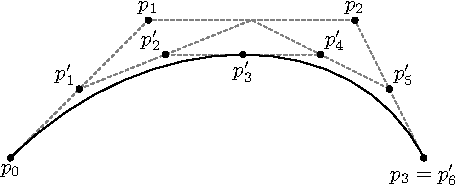
\includegraphics{subdivision}
%	     \caption{A Figure}
%	 \label{subd}
%	\end{figure}

%\clearpage %% starts a new page and stops trying to place floats such as tables and figures

%\section{More Figure Stuff}
%You can also scale and rotate figures.
% 	\begin{figure}[h!]
	   
%	       \centering
	    % DO NOT ADD A FILENAME EXTENSION TO THE GRAPHIC FILE
%	    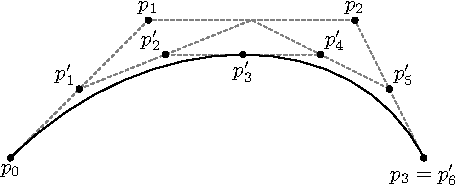
\includegraphics[scale=0.5,angle=180]{subdivision}
	    % if your figure shows up not where you want it, it may just be too big to fit. You can use the scale argument to shrink it, e.g. scale=0.85 is 85 percent of the original size. 
%	     \caption{A Smaller Figure, Flipped Upside Down}
%	 \label{subd2}
%	\end{figure}

%\section{Even More Figure Stuff}
%With some clever work you can crop a figure, which is handy if (for instance) your EPS or PDF is a little graphic on a whole sheet of paper. The viewport arguments are the lower-left and upper-right coordinates for the area you want to crop.

% 	\begin{figure}[h!]
%	    	       \centering
%	    % DO NOT ADD A FILENAME EXTENSION TO THE GRAPHIC FILE
%	   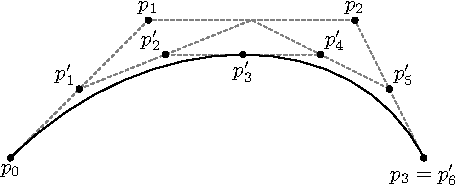
\includegraphics[clip=true, viewport=.0in .0in 1in 1in]{subdivision}
%	    \caption{A Cropped Figure}
%	 \label{subd3}
%	\end{figure}
%	
%      \subsection{Common Modifications}
%      The following figure features the more popular changes thesis students want to their figures. This information is also on the web at \url{web.reed.edu/cis/help/latex/graphics.html}.
%           \renewcommand{\thefigure}{0.\arabic{figure}} %Renumbers the figure to the type 0.x
%    \addtocounter{figure}{4} %starts the figure numbering at 4
%    \begin{figure}[htbp]
%    \begin{center}
%   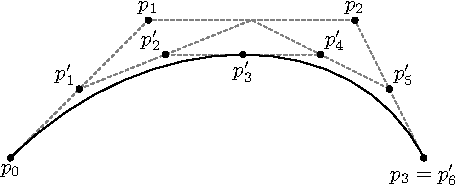
\includegraphics[scale=0.5]{subdivision}
%    \caption[Flower type and percent specialization]{\footnotesize{Interaction bar plot showing the degree of specialization for each flower type.}} %the special ToC caption is in square brackets. The \footnotesize makes the figure caption smaller
%    \label{barplot}
%    \end{center}
%    \end{figure} 

%\chapter*{Conclusion}
%         \addcontentsline{toc}{chapter}{Conclusion}
%	\chaptermark{Conclusion}
%	\markboth{Conclusion}{Conclusion}
%	\setcounter{chapter}{4}
%	\setcounter{section}{0}
	
%Here's a conclusion, demonstrating the use of all that manual incrementing and table of contents adding that has to happen if you use the starred form of the chapter command. The deal is, the chapter command in \LaTeX\ does a lot of things: it increments the chapter counter, it resets the section counter to zero, it puts the name of the chapter into the table of contents and the running headers, and probably some other stuff. 

%So, if you remove all that stuff because you don't like it to say ``Chapter 4: Conclusion'', then you have to manually add all the things \LaTeX\ would normally do for you. Maybe someday we'll write a new chapter macro that doesn't add ``Chapter X'' to the beginning of every chapter title.

%\section{More info}
%And here's some other random info: the first paragraph after a chapter title or section head \textit{shouldn't be} indented, because indents are to tell the reader that you're starting a new paragraph. Since that's obvious after a chapter or section title, proper typesetting doesn't add an indent there. 


%If you feel it necessary to include an appendix, it goes here.
    \appendix
     \chapter{Comparison Tables}
     \begin{longtable}{lcc}
\caption[Original and Replication Results]{This is a complete table of results for comparison between the original and replication studies.}\\
\hline
\large{Result} & \large{Original} & \large{Replication} \\
\hline
\endfirsthead

\multicolumn{3}{l}%

{\tablename\ \thetable\ -- \textit{Continued from previous page}} \\
\hline
\large{Result} & \large{Original} & \textbf{Replication} \\
\hline
\endhead
\hline \multicolumn{3}{l}{\textit{Continued on next page}} \\


\endfoot
%\line
\endlastfoot
\bf{Startle} & & \\
ANOVA: Mean Startle & &\\
Magnitude by Trial Type & \textit{F}(2,60)=5.64, \textit{p} < .05 & \textit{F}(2,56) = 9.36, \textit{p} < .001\\
\\
\textit{t} test: Startle (Error) versus & & \\
Startle (Correct Predictable) & \textit{t}(30) = 2.51, \textit{p} < .01 & \textit{t}(28) = 3.79, \textit{p} < .001\\
\\
\textit{t} test: Startle (Error) versus & & \\
Startle (Correct Unpredictable) & \textit{t}(30) = 2.61, \textit{p} < .01 & \textit{t}(28) = 2.90, \textit{p} < .01\\
\\
\textit{t} test: Startle (Correct Predictable) & & \\
versus Startle (Correct Unpredictable) & \textit{t}(30) = 0.99, \textit{p} > .30 & \textit{t}(28) = -1.72, \textit{p} > .05\\
\\
\bf{ERN} & & \\
\textit{t} test: ERN difference from 0 & \textit{t}(30) = 3.83, \textit{p} < .001 & \textit{t}(29) = -6.85, \textit{p} < .001\\
\\
\bf{EPS-ERN correlation} & & \\
Correlation between EPS and ERN & \textit{r} = .38, \textit{p} < .05 & \textit{r} = .28, \textit{p} > .05\\
Correlation After Median Split & \textit{r} = -.60, \textit{p} < .05 & \textit{r} = -.56, \textit{p} < .03\\
\bottomrule
\end{longtable}
\chapter{Free and Open Source Software Used}
The only licensed software used was Presentation, for presentation of stimuli, Brain Vision Recorder, and Analyzer. The electrodes amplifiers converted the signal from analog to digital, Brain Vision Recorder collected raw EEG and data trigger codes from Presentation, and Analyzer was used for EEG preprocessing.\\
See The Future of Open Science for a discussion of FOSS.
\begin{table}[htdp] % begins the table floating environment. This enables LaTeX to fit the table where it works best and lets you add a caption.
\caption{Free (F) and Open Source (OS) Software Used.} 
% The words in square brackets of the caption command end up in the Table of Tables. The words in curly braces are the caption directly over the table.
\begin{center} 
% makes the table centered
\begin{tabular}{cccc} 
% the tabular environment is used to make the table itself. The {c c c c} specify that the table will have four columns and they will all be center-aligned. You can make the cell contents left aligned by replacing the Cs with Ls or right aligned by using Rs instead. Add more letters for more columns, and pipes (the vertical line above the backslash) for vertical lines. Another useful type of column is the p{width} column, which forces text to wrap within whatever width you specify e.g. p{1in}. Text will wrap badly in narrow columns though, so beware.
\toprule % a horizontal line, slightly thicker than \hline, depends on the booktabs package
Purpose & Software & License & Status \\ % the first row of the table. Separate columns with ampersands and end the line with two backslashes. An environment begun in one cell will not carry over to adjacent rows.
  \midrule % another horizontal line
typesetting & LaTeX & LaTeX Project Public License & F/OS\\
reference management & BibDesk & Berkeley Software Distribution & F/OS\\
bibliographic data & Zotero & Affero General Public License & F/OS\\
data analysis & R & GNU General Public License & F/OS\\
version control & Git & GNU General Public License & F/OS\\
\bottomrule % yet another horizontal line
\end{tabular}
\end{center}
Code for this experiment can be found at \url{github.com/meli-lewis/} .\\
\label{tab:FOSS} % labels are useful when you have more than one table or figure in your document. See our online documentation for more on this.
\end{table}

%     \begin{longtable}[||c|c|c||] % begins the table floating environment. This enables LaTeX to fit the table where it works best and lets you add a caption.
%\caption{Results: Original and Replication} 
% The words in square brackets of the caption command end up in the Table of Tables. The words in curly braces are the caption directly over the table.
%\begin{center} 
% makes the table centered
%\begin{tabular}{l l l} 
% the tabular environment is used to make the table itself. The {c c c c} specify that the table will have four columns and they will all be center-aligned. You can make the cell contents left aligned by replacing the Cs with Ls or right aligned by using Rs instead. Add more letters for more columns, and pipes (the vertical line above the backslash) for vertical lines. Another useful type of column is the p{width} column, which forces text to wrap within whatever width you specify e.g. p{1in}. Text will wrap badly in narrow columns though, so beware.
%\toprule % a horizontal line, slightly thicker than \hline, depends on the booktabs package
%  Relationship & Original & Replication \\ % the first row of the table. Separate columns with ampersands and end the line with two backslashes. An environment begun in one cell will not carry over to adjacent rows.
%  \midrule % another horizontal line

%Number of Errors & 23.29 $SD=9.68$) & 36.13 \textit{SD}=19.70) \\
%\\
%\bf{Startle} & & \\ % another row
%ANOVA: Mean Startle Magnitude & & \\
%by Trial Type & \textit{F}(2,60)=5.64, \textit{p} < .05 & \textit{F}(2,56) = 9.36, \textit{p} < .001\\
%\\
%\textit{t} test: Startle (Error) versus & & \\
%Startle (Correct Predictable) & \textit{t}(30) = 2.51, \textit{p} < .01 & \textit{t}(28) = 3.79, %\textit{p} < .001\\
%\\
%\textit{t} test: Startle (Error) versus & & \\
%Startle (Correct Unpredictable) & \textit{t}(30) = 2.61, \textit{p} < .01 & \textit{t}(28) = 2.90, \textit{p} < .01\\
%\\
%\textit{t} test: Startle (Correct Predictable) & & \\
%versus Startle (Correct Unpredictable) & \textit{t}(30) = 0.99, \textit{p} > .30 & \textit{t}(28) = -1.72, \textit{p} > .05\\
%\\
%\bf{ERN} & & \\
%\textit{t} test: ERN difference from 0 & \textit{t}(30) = 3.83, \textit{p} < .001 & \textit{t}(29) = -6.85, \textit{p} < .001\\
%\bf{EPS-ERN correlation} & & \\
%\bottomrule % yet another horizontal line
%\end{tabular}
%\end{center}
%\label{inheritance} % labels are useful when you have more than one table or figure in your document. See our online documentation for more on this.
%\end{longtable}

      \chapter{Report to the Reproducibility Project} \label{chap:RPreport}%\section{Report to the Reproducibility Project} \label{sec:RPreport}
     \begin{center}
     \begin{large}
Replication of ``Errors Are Aversive"\\
by Greg Hajcak \& Dan Foti\\
(2008, \textit{Psychological Science})\\
      Melissa Lewis and Michael Pitts\\
      mlewis@reed.edu\\
      mpitts@reed.edu\\
      \end{large}
      \end{center}
      \section{Introduction}
      The error-related negativity (ERN) is a negative-going event-related potential component that peaks very quickly after a commission error, and owing to its modulation by affective state and its maximal location being over the anterior cingulate cortex, could be functionally related to a defensive motivational state. That is, it may have some relationship to physiological responses associated with the organism being in danger. The human startle response is a specific measure of defensive state and is often measured by blink response at the orbicularis muscle just below the eye. If such a stable measure of defensive motivation is correlated to the ERN in magnitude, it suggests the latter's functional role in defensive motivation.
      
      The original experiment demonstrated both that people's startle response to a loud auditory stimulus is greater when they have just committed an error and that the magnitude of this response is correlated to the amplitude of the ERN.
      \section{Methods}
      \subsection{Power Analysis}
      Because the main finding of the original study was a correlation of .38, p < .05, one-tailed, and I am to meet a power of .8, I will run 42 subjects.
      \subsection{Planned Sample}
      Sample will be 18-35 years old, with normal or corrected-to-normal vision and no history of neurological disorders.
      \subsection{Materials}
      ``Continuous electroencephalographic (EEG) and electromyographic (EMG) activity was recorded using an ActiveTwo head cap and the ActiveTwo BioSemi system (BioSemi, Amsterdam, The Netherlands)."
      
     We used the EasyCap electrode cap and BrainAmps Standard system (Brain Products, Gilding, Germany).
      
      ``Recordings were taken from 64 scalp electrodes based on the ten-twenty system, as well as from two electrodes placed on the left and right mastoids. The electrooculogram (EOG) generated from blinks and eye movements was recorded from four facial electrodes: two approximately 1 cm above and below the participant�s right eye, one approximately 1 cm to the left of the left eye, and one approximately 1 cm to the right of the right eye."
      
      We used caps with 96 scalp electrodes at equidistant positions as well as from two reference electrodes placed on the left and right mastoids. EOG was recorded identically. 
      
      ``The startle response was measured with two electrodes placed approximately 12 mm apart under the participant�s left eye on the obicularis muscle. As per BioSemi�s design, the ground electrode during acquisition was formed by the Common Mode Sense active electrode and the Driven Right Leg passive electrode. All bioelectric signals were digitized on a laboratory microcomputer using ActiView software (BioSemi). Sampling was at 1024 Hz."
      
     	EMG electrodes were placed under the eye and 12mm apart. Though the original article did not describe their placement except in reference to the other, the medial electrode was placed under the pupil and the lateral electrode was placed 12mm to the right of it, as per Hajcak's directions in an email correspondence. His directions about vertical placement of the electrodes were to feel the orbicularis muscle for where the blink is maximal. All bioelectric signals were digitized on a laboratory microcomputer using Recorder software (Brain Products). Sampling was at the rate allowable by the software, 1000 Hz.
	\subsection{Procedure}
	``The task was an arrow version of the flankers task (cf. Hajcak et al., 2005). On each trial, five horizontally aligned arrowheads were presented, and participants had to respond to the direction of the central arrowhead by pressing the left or right mouse button. On compatible trials, all five arrowheads pointed in the same direction (either left or right), and on incompatible trials, the central arrowhead pointed in the direction opposite the direction of the flanking arrowheads. Compatible and incompatible trials were equally frequent, and all stimuli were presented for 200 ms with an intertrial interval that varied randomly from 500 to 1,000 ms. Participants performed eight blocks of 30 trials. At the end of each block, participants received performance feedback designed to encourage fast and accurate responding. If performance was 75\% correct or lower, the message `Please try to be more accurate' was displayed; performance above 90\% correct was followed by `Please try to respond faster'; if performance was between these levels, the message `You're doing a great job' was displayed. All participants performed one practice block of 30 trials.'"
	
	I was unable to obtain the Presentation code from Hajcak, but wrote my own and when I sent it to him, he approved it.
      \subsection{Analysis Plan}
      Analysis was identical to that of the original study except in the software used and in the sampling rate (1000 Hz rather than 1024 Hz).\\
Offline analysis was performed using Brain Vision Analyzer software (Brain Products, Gilching, Germany). Data was referenced to the numeric mean of the mastoids and band-pass filtered with cutoffs of 0.1 and 30 Hz. EEG was segmented for each trial, beginning 200 ms before response and continuing for 800 ms. It was corrected for blinks and eye movements using EMCP.  The ERN was defined as the average activity in a 0- to 100-ms window following response onset on error trials, but it generally peaks approximately 50 ms following commission of an error. The ERN was statistically evaluated using R, with Greenhouse-Geisser correction applied to p values associated with multiple degrees of freedom, repeated measures comparisons.

Startle response EMG data will be band-pass filtered (28�512 Hz; 24 dB/ octave roll-off), rectified, then low-pass filtered at 30 Hz (24 dB/ octave) and baseline-corrected. Response magnitude and latencies will be quantified according to a peak in the 20- to 120-ms window after the startle probe was presented. It will be statistically evaluated with Greenhouse-Geisser correction applied to p values associated with multiple degrees of freedom, repeated measures comparisons. However, it was studied with R rather than with SPSS as in the original study.
Participants were excluded only if their averages following correction contain artifacts of high reference or ground impedance and/or facial movement disrupting a potential signal.
      \subsection{Differences from Original Study}
      Differences in materials were outlined in the above materials section. The original article did not specify an age range, but the age range for this study was 18-35. The original author analyzed data using SPSS, while this data was analyzed with R. The original article described the auditory stimulus as being 105dB, where in this study the speakers could only go up to 99dB.




%This is where endnotes are supposed to go, if you have them.
%I have no idea how endnotes work with LaTeX.

  \backmatter % backmatter makes the index and bibliography appear properly in the t.o.c...



% if you're using bibtex, the next line forces every entry in the bibtex file to be included
% in your bibliography, regardless of whether or not you've cited it in the thesis.
\bibliography{thesis}                                                                                                                                                \bibliographystyle{APA/apa-good}                                                                                                                                                                              %\nocite{*}
% Finally, an index would go here... but it is also optional.
\end{document}
